\subsection{Teorema de Bolzano-Weierstrass y el teorema de Cantor}

Ahora, lo que queremos es ver cuándo $A \subset \R^n$ tiene puntos de acumulación.

\begin{defn}
    Diremos que el conjunto $A \subset \R^n$ es \ul{acotado} si $\exists M > 0$ tal que $A \subset B_2(0, M)$.
\end{defn}

\begin{teo}[Bolzano-Weierstrass]\label{teo:BW}
    Si $A \subset \R^n$ es acotado y contiene una cantidad infinita de puntos. Entonces $A' \neq \emptyset$.
\end{teo}

\begin{proof}
    Como $A$ es acotado, entonces existe $M > 0$ tal que
    
    \[
    A \subset J_1 = \prod_{i=1}^n [-M,M]
    \]
    
    \noindent donde $J_1 = \{x \in \R^n : |x_i| \leq M, \forall i = 1, \dots, n\}$.
    
    Adicionalmente, podemos considerar a $J_1$ como $J_1 = \prod_{i=1} I_i^{(1)}$ donde $I_i^{(1)} = [-M,M]$. Ahora subdividiremos cada $I_i^{(1)}$ en dos intervalos
    
    \[
    I_{i,1}^{(1)} = [-M,0], \quad I_{i,2}^{(1)} = [0, M]
    \]
    
    \noindent para todo $i = 1, \dots, n$.
    
    \begin{marginfigure}
        \centering
        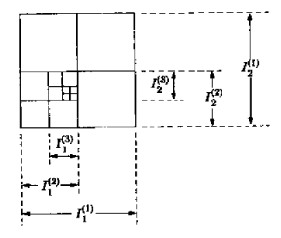
\includegraphics[scale=0.5]{img/I_2.png}
        \caption{\footnotesize{Imagen sacada del Apostol. Representación para cuando $\R^2$. Lo que queremos son todas las posibles combinaciones para $I_{1,k}^{(1)}$, $I_{2,k}^{(1)}$ (con $k=1$ y $k=2$). Es decir, todos los cuadrados posibles que se pueden formar al picar el cuadrado más grande por la mitad de forma vertical y horizontal (para $\R^2$ tenemos 4 posibles cuadrados).}}
        \label{fig:R^2}
    \end{marginfigure}
    
    Ahora, consideremos todos los productos de la forma
    
    \[
    I_{1,k_1}^{(1)} \times I_{2,k_1}^{(1)} \times \dots \times I_{n,k_n}^{(1)} \quad \text{con $k_i=1,2$}
    \]
    
    En total, existen $2^n$ productos de este tipo (por que hay dos posibles intervalos para cada $I_i$ con $i = 1, \dots, n$) y cada uno de ellos da como resultado un intervalo $n$-dimensional. Como la unión de estos $2^n$ intervalos es $J_1$ y $J_1$ contiene una cantidad infinita de puntos de $A$, entonces al menos un $J_2 = I_{j, k_j}^{(1)}$ que contiene una cantidad infinita de elementos de $A$. Este intervalo puede ser expresado como
    
    \[
    J_2 = \prod_{i=1} I_i^{(2)}
    \]
    
    \noindent donde cada $I_k^{(2)}$ es un subintervalo de $I_k^{(1)}$.
    
    Igual que antes, al bisecar cada uno de estos subintervalos, podemos encontrar un intervalo $n$-dimensional $J_3$ que contiene una cantidad infinita de puntos de $A$. Continuando este proceso, encontraremos una familia contable de intervalos $n$-dimensionales $J_1, J_2, J_3, \dots$ tales que el $m$-ésimo intervalo $J_m$ tiene infinitos puntos de $A$ y se puede expresar de la forma
    
    \[
    J_m = I_1^{(m)} \times I_2^{(m)} \times \dots \times I_n^{(m)} \quad \text{donde $I_k^{(m)} \subseteq I_k^{(1)}$}
    \]
    
    \noindent y además los $I_k^{(m)}$ son de la forma $I_k^{(m)} = [a_k^m, b_k^m]$. Y para cada uno de ellos su longitud es\marginfootnote{Recordemos que por cada "nivel" estamos bisecando los intervalos.}
    
    \[
    \left|b_k^{(m)} - a_k^{(m)}\right| = \frac{M}{2^{m-2}} \quad \text{donde $k = 1, \dots, n$}
    \]
    
    Observamos que la sucesión $\{a_k^{(m)}\}_{m=1}^{\infty}$ es creciente y al hacer $n \rightarrow \infty$, ella va a tender a $\sup_{m \geq 1} a_k$. Análogamente la sucesión $\{b_k^{(m)}\}_{m=1}^{\infty}$ es decreciente y al hacer $n \rightarrow \infty$, ella va a tender a $\inf_{m \geq 1} b_k^{(m)}$. Luego para cada $k$, estos valores coinciden en un valor en común $t_k$ al hacer $n \rightarrow \infty$.
    
    Sea $t = (t_1, t_2, \dots, t_n)$. Consideremos $B_2(t, r)$ para $r > 0$. Este punto $t$ está contenido en cada uno de los intervalos $J_1, J_2, \dots$ construídos anteriormente. Entonces cuando $m$ es tal que $M/2^{m-2} < r/2$ tneemos que la bola $B_2(t, r)$ contiene a $J_m$. Pero $J_m$ contiene una cantidad infinita de puntos de $A$ por construcción, entonces
    
    \[
    \left( B_2(t, r) \backslash \{t\} \right) \cap A \neq \emptyset
    \]
    
    Por lo tanto, $t$ es un punto de acumulación de $A$, y de esta forma queda demostrado.
\end{proof}

\begin{teo}[Cantor]
    Sea $(\Oc_j)_{j=1}^{\infty} \subset \R^n$ tal que
    
    \begin{itemize}
        \item $\Oc_{j+1} \subset \Oc_j$ para cada $j \geq 1$.
        \item $\Oc_j$ es cerrado, acotado y contiene infinitos elementos.
    \end{itemize}
    
    Entonces $\bigcap_j \Oc_j$ es cerrado y no-vacío.
\end{teo}

\begin{proof}
    Denotaremos por
    
    \[
    S = \bigcap_j \Oc_j
    \]
    
    Como $S$ es una intersección arbitraria de conjuntos cerrados, entonces es cerrado.
    
    Nos queda ver que $S$ es no-vacío. Como cada $\Oc_j$ es un conjunto con una cantidad infinita de elementos, entonces podemos definir
    
    \[
    A = \{x_1, x_2, \dots, x_j, \dots\} \quad \text{con $x_j \in \Oc_j$}
    \]
    
    Observamos que $A \subset \Oc_j$ ya que al tener $\Oc_{j+1} \subset \Oc_j$, entonces $x_1, \dots \in \Oc_1$. Como $\Oc_1$ es acotado, existe $M > 0$ tal que
    
    \[
    A \subset \Oc_1 \subset B(0, M)
    \]
    
    \noindent lo que implica que $A$ es acotado.
    
    Hemos verificado entonces que $A$ tiene infinitos elementos y $A$ es acotado. Entonces, por el teorema de Bolzano-Weierstrass, $A' \neq \emptyset$. Sea $a \in A'$, luego cada entorno de $a$ contiene una cantidad infinita de puntos de $A$ los cuales pertenecen a $\Oc_j$ (para cada $j$), salvo posiblemente una cantidad finita de ellos. Entonces este entorno también contiene una cantidad infinita de puntos de $\Oc_j$, por lo que $a \in \Oc_j'$. Pero como cada $\Oc_j$ es cerrado, entonces $a \in \Oc_j' = \Oc_j$ para todo $j$. Por lo tanto $a \in S$ y $S \neq \emptyset$.
    
    De esta manera queda demostrado.
\end{proof}

\subsection{Recubrimientos en $\R^n$}

\begin{defn}
    Una familia $\F = (A_j)_{j=1}^{\infty}$, tal que $A_j \subset \R^n$ y $A_j \neq \emptyset$ es un \ul{recubrimiento} de un conjunto $S \subset \R^n$ si $S \subset \bigcup_j A_j$.
    
    Si además, cada $A_j$ es abierto, decimos que el recubrimiento es por abiertos. Si cada $A_j$ es cerrado, decimos que el recubrimiento es por cerrados.
\end{defn}

\begin{teo}[Heine-Borel]
    Sea $\F$ un recubrimiento por abiertos de $A$, con $A$ cerrado y acotado en $\R^n$. Entonces hay una subcolección finita de $\F$ que cubren a $A$.
\end{teo}

\begin{proof}
    Denotemos a la familia de esta manera:
    
    \[
    \F = \left( I_j \right)_j \quad \text{tal que} \quad A \subset \bigcup_j I_j
    \]
    
    \noindent donde cada $I_j$ es abierto.
    
    Ahora definamos para cada $m \geq 1$ la unión
    
    \[
    S_m = \bigcup_{j=1}^m I_j
    \]
    
    Como cada $S_m$ es una unión arbitraria de abiertos, entonces $S_m$ es abierto. Por lo tanto $S_m^c = \R^n \backslash S_m$ es cerrado. Sean ahora $\{ \Oc_m \}_{m=1}^{\infty}$ tales que
    
    \[
    \Oc_1 = A, \qquad \Oc_m = A \cap S_m^c, \quad \text{si $m > 1$}
    \]
    
    Supongamos que $\Oc_m \neq \emptyset$ para todo $m$. Observemos que $\Oc_j = A \cap S_m^c$, y como $S_m$ crece, entonces $S_m^c$ decrece, por lo tanto $\{ \Oc_m \}_{m=1}^{\infty}$ decrece. Entonces tenemos que $\Oc_{m+1} \subset \Oc_m$ para todo $m$.
    
    Adicionalmente, también tenemos que
    
    \begin{itemize}
        \item Cada $\Oc_m$ es cerrado porque es la intersección de dos conjuntos cerrados.
        \item Cada $\Oc_m$ es acotado porque es la intersección de $S_m^c$ con el conjunto acotado $A$.
    \end{itemize}
    
    Entonces, por el teorema de Cantor, entonces $\bigcap_m \Oc_m \neq \emptyset$. Por lo tanto $\exists x_0$ tal que $x_0 \in A \wedge x_0 \in S_m^c$ para todo $m$. Esto implica que $x_0 \in A \wedge x_0 \notin S_m$ para todo $m$. Pero esto contradice el hecho de que $\F$ es un cubrimiento de $A$ ya que $A \subset_j I_j \subseteq \bigcup_k S_k$.
    
    Por lo tanto, existe algún $m_0$ para el cual $\Oc_{m_0} = \emptyset$. Lo cual implica que
    
    \[
    S_{m_0}^c \cap A = \emptyset \implies A \subset S_{m_0} = \bigcup_{j=1}^{m_0} I_j
    \]
    
    De esta forma, queda demostrado.
\end{proof}

\begin{defn}
    Un conjunto $A \subset \R^n$ es \ul{compacto} sii de todo cubrimiento por abiertos de $A$, podemos extraer un subcubrimiento finito.
\end{defn}

\begin{teo}
    Si $A \subset \R^n$ es compacto. Entonces $A$ es cerrado y acotado.
\end{teo}

\begin{proof}
    Sea $p \in A$ y consideremos la colección de $n$-bolas
    
    \[
    F = \{ B(p, k) \}_{k=1}^{\infty}
    \]
    
    \noindent donde $B(p, k) = \{ y \in \R^n : \normaeuc{y-p} < k \}$.
    
    Luego $A \subset \bigcup_{p \in A} \bigcup_{k=1}^{\infty} B(p, k)$. Pero $A$ es compacto, entonces existe al menos un $m_0 \in \N$ tal que
    
    \[
    A \subset \bigcup_{k=1}^{m_0} B(p, k)
    \]
    
    Como todas estas bolas son concéntricas, entonces
    
    \[
    A \subset \bigcup_{k=1}^{m_0} B(p, k) \subseteq B(p, m_0) \implies A \subset B(p, m_0)
    \]
    
    De esta forma, $A$ es un conjunto acotado, y queda verificar que $A$ es cerrado: Supongamos entonces que $A$ no es cerrado, entonces existe un elemento $y \in A'$ tal que $y \notin A$. Sea $x \in A$ y denotemos por $r_x = \normaeuc{x - y} / 2$. Luego la familia $\{ B_2(x, r_x) : x \in S \}$ es cubrimiento por abiertos de $A$. Pero $A$ es compacto, entonces hay una cantidad finita $n \in \N$ de estos entornos tales que la unión de ellos cubren a $A$, luego
    
    \[
    A \subset \bigcup_{k=1}^n B(x_k, r_{x_k})
    \]
    
    Consideremos $r = \min_{k=1, \dots, n} (r_k)$. Entonces
    
    \[
    B(y, r) \cap B(x_k, r_{x_k}) = \emptyset \quad \text{para todo $k=1, \dots, n$}
    \]
    
    En efecto es vacío, ya que si
    
    \[
    x \in B(y, r) \implies \normaeuc{x-y} < r \geq r_{x_k} \quad \text{para todo $k$}
    \]
    
    Y por la desigualdad triangular, tenemos que $\normaeuc{y-x_k} \leq \normaeuc{y-x} + \normaeuc{x - x_k}$. Luego
    
    \[
    \normaeuc{x - x_k} \geq \normaeuc{y-x_k} - \normaeuc{x-y} = 2r_k - \normaeuc{x-y} > r_k
    \]
    
    Y esto implica que $x \notin B_2(x_k, r_k)$. Entonces nos queda que
    
    \[
    B(y, r) \cap B(x_k, r_{x_k}) = \emptyset \quad \text{para todo $k=1, \dots, n$}
    \]
    
    Pero ya establecimos que $\bigcup_{k=1}^n B(x_k, r_{x_k})$ es un cubrimiento por abiertos de $A$. Entonces lo anterior implica que
    
    \[
    B(y, r) \cap A = \emptyset
    \]
    
    Luego $y$ no es punto de acumulación de $A$. Esto es una contradicción, ya que establecimos que $y \in A'$. Como estamos partiendo del hecho de suponer que $A$ no es cerrado, entonces necesariamente $A$ tiene que ser cerrado.
    
    De esta forma, queda demostrado que $A$ es cerrado y acotado.
\end{proof}